% !TeX program = xelatex
% 实验设计流程图（精简版）：两臂 × 三个比较层级
% 编译：xelatex -interaction=nonstopmode -halt-on-error experiment_design_flowchart.tex
% 插图：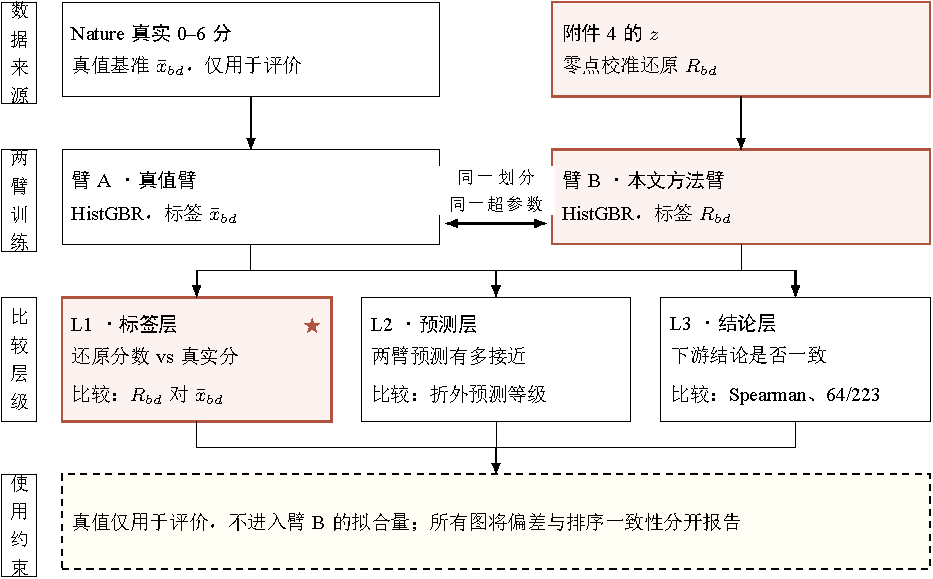
\includegraphics[width=\linewidth]{experiment_design_flowchart.pdf}
\documentclass[tikz,border=0pt]{standalone}
\usepackage[UTF8,fontset=windows]{ctex}
\usepackage{amsmath,amssymb}
\usetikzlibrary{arrows.meta,calc}
\setmainfont{Times New Roman}
\definecolor{B0543F}{HTML}{B0543F}
\definecolor{FCF3F0}{HTML}{FCF3F0}
\definecolor{FFFDF4}{HTML}{FFFDF4}
\newcommand{\ttl}[1]{{\heiti #1}}
\begin{document}
\begin{tikzpicture}[x=1mm,y=-1mm,>=Latex,
  line width=0.45pt,
  box/.style={draw,rectangle,anchor=north west,inner sep=1.6mm,outer sep=0pt,
              align=left,font=\songti\fontsize{9.4}{12}\selectfont},
  accent/.style={box,draw=B0543F,line width=0.7pt,fill=FCF3F0},
  note/.style={box,dashed,fill=FFFDF4,line width=0.5pt},
  side/.style={draw,rectangle,anchor=north west,inner sep=0pt,outer sep=0pt,
               text width=5.8mm,align=center,font=\songti\fontsize{9}{10.5}\selectfont},
  edge/.style={->,line width=0.55pt},
  both/.style={<->,line width=0.6pt},
  small/.style={font=\songti\fontsize{8.4}{10}\selectfont,fill=white,inner sep=0.4mm}]
\path[use as bounding box] (0,0) rectangle (158,98);

% ============ 1. 标签来源 ============
\node[side,minimum height=16mm] at (0.3,0.3) {数\\据\\来\\源};
\node[box,text width=60.8mm,minimum height=16mm] (srcA) at (10.5,0.3)
  {\ttl{Nature 真实 0--6 分}\\
   真值基准 $\bar x_{bd}$，仅用于评价};
\node[accent,text width=60.8mm,minimum height=16mm] (srcB) at (93.5,0.3)
  {\ttl{附件 4 的 $z$}\\
   零点校准还原 $R_{bd}$};

% ============ 2. 两臂 ============
\node[side,minimum height=16mm] at (0.3,25.3) {两\\臂\\训\\练};
\node[box,text width=60.8mm,minimum height=16mm] (armA) at (10.5,25.3)
  {\ttl{臂 A · 真值臂}\\
   HistGBR，标签 $\bar x_{bd}$};
\node[accent,text width=60.8mm,minimum height=16mm] (armB) at (93.5,25.3)
  {\ttl{臂 B · 本文方法臂}\\
   HistGBR，标签 $R_{bd}$};
\draw[both] (75.5,37.8) -- (92.5,37.8);
\node[small,align=center,text width=19mm,anchor=south] at (84,36.3)
  {同一划分\\同一超参数};

% ============ 3. 比较层级 ============
\node[side,minimum height=21mm] at (0.3,50.3) {比\\较\\层\\级};
\node[accent,text width=42.4mm,minimum height=21mm] (L1) at (10.5,50.3)
  {\ttl{L1 · 标签层}\hfill{\color{B0543F}$\bigstar$}\\
   还原分数 vs 真实分\\[1mm]
   比较：$R_{bd}$ 对 $\bar x_{bd}$};
\node[box,text width=42.4mm,minimum height=21mm] (L2) at (61.2,50.3)
  {\ttl{L2 · 预测层}\\
   两臂预测有多接近\\[1mm]
   比较：折外预测等级};
\node[box,text width=42.4mm,minimum height=21mm] (L3) at (111.9,50.3)
  {\ttl{L3 · 结论层}\\
   下游结论是否一致\\[1mm]
   比较：Spearman、64/223};

% ============ 4. 约束 ============
\node[side,minimum height=16mm] at (0.3,80.3) {使\\用\\约\\束};
\node[note,text width=143.8mm,minimum height=16mm] (note) at (10.5,80.3)
  {真值仅用于评价，不进入臂 B 的拟合量；所有图将偏差与排序一致性分开报告};

% ============ 连线 ============
\draw[edge] (42.5,16.3) -- (42.5,25.3);           % 来源 → 臂A
\draw[edge] (125.5,16.3) -- (125.5,25.3);         % 来源 → 臂B
\draw (42.5,41.3) -- (42.5,45.8);                 % 臂A ↓
\draw (125.5,41.3) -- (125.5,45.8);               % 臂B ↓
\draw (33.3,45.8) -- (134.7,45.8);                % 汇聚横线
\draw[edge] (33.3,45.8) -- (33.3,50.3);           % → L1
\draw[edge] (84.0,45.8) -- (84.0,50.3);           % → L2
\draw[edge] (134.7,45.8) -- (134.7,50.3);         % → L3
\draw (33.3,71.3) -- (33.3,75.8);                 % L1 ↓
\draw (84.0,71.3) -- (84.0,75.8);                 % L2 ↓
\draw (134.7,71.3) -- (134.7,75.8);               % L3 ↓
\draw (33.3,75.8) -- (134.7,75.8);                % 汇聚横线
\draw[edge] (84.0,75.8) -- (84.0,80.3);           % → 约束
\end{tikzpicture}
\end{document}
